\quad \quad Firstly, good job on finishing chapter 1, it is not an easy feat. Stepping into this chapter, you may feel overwhelmed by the name, \textit{Linear Algebra}. What is that? Is that algebra but somehow in a linear way? We will discuss both the theoretical and practical aspects of Linear Algebra. Please take note though, the knowledge in this chapter will not be used until Calculus III to IV in part IV of the book. If you are just willing to learn Calc I and II, you do not need the knowledge here. With that said, let's delve into Vectors. A concept that is very ubiquitous in this world is a coordinate, like the GPS coordinate in the maps app. A coordinate simply describes the position of a point in space. Generally, it is denoted \((x,y)\) in 2 dimensions and \((x,y,z)\) in 3 dimensions. Likewise, vectors are also behaves like coordinates and are written down in a \textit{similar} fashion. Think of a vector as an arrow pointing to a coordinate.
\begin{definition}
  A vector is a mathematical object with a magnitude, or length, and a direction. A vector, \(\vec{a}\) , pointing to the coordinate \((x,y)\) is denoted as:
  \begin{equation*}
    \vec{a} = \begin{bmatrix}
                x \\
                y
              \end{bmatrix} 
  \end{equation*}
  \marginnote{\footnotesize \textit{Likewise, a vector pointing to the coordinate \((x,y,z)\) is denoted \(
    \begin{bsmallmatrix}
      x \\
      y \\
      z
    \end{bsmallmatrix}
\)}}
\end{definition}


Of course, vectors by themselves are not very useful. Hence, we shall define the vector space. For the purposes of this text, you may think of vector spaces as the 2 and 3 dimensional euclidean spaces you are very familiar with. In a vector space, we can finally meaningfully manipulate them. Take a look at the vector \( \vec{a}=
  \begin{bsmallmatrix}
    1 \\
    2
  \end{bsmallmatrix}
  \) and the vector \( \vec{b}=
  \begin{bsmallmatrix}
    -2 \\
    1
  \end{bsmallmatrix}
\) in the two dimensional euclidean space:
\begin{figure}[h]
  \centering
  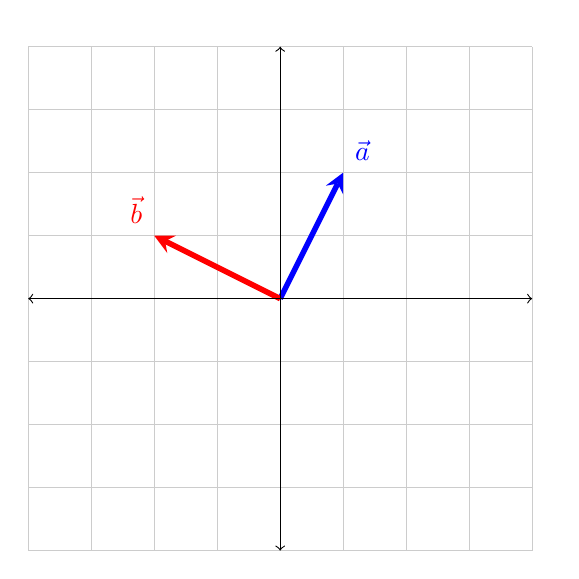
\begin{tikzpicture}[scale=0.8]
    \draw[thin, gray!40] (-4,-4) grid (4,4);
    \draw[line width=2pt, blue, -stealth] (0,0) -- (1,2) node[anchor=south west]{\(\vec{a}\)};
    \draw[line width=2pt, red, -stealth] (0,0) -- (-2,1) node[anchor=south east]{\(\vec{b}\)};
    \draw[<->] (-4,0) -- (4,0) node[right]{\(\ihat\)};
    \draw[<->] (0,-4) -- (0,4) node[above]{\(\jhat\)};
  \end{tikzpicture}
  \caption{Figure of vectors \(\vec{a}\) and \(\vec{b}\).}
  \label{vecab}
\end{figure}


You may have noticed that the coordinate axes in \Cref{vecab} are unusual. Instead of the usual \(x\) axes, you have the \(\ihat\) and \(\jhat\) axes. This is a convention in linear algebra. \(\ihat\) translates to the \(x\) axis and \(\jhat\) translates to the \(y\) axis. Likewise, in the third dimension, \(\khat\) represents the \(z\) axis. With this in mind, another way of writing a vector \(\vec{a}=
\begin{bsmallmatrix}
  x \\
  y 
\end{bsmallmatrix} \) is \(\vec{a}=x \ihat + y \jhat \). Of course, vectors by themselves might not be that useful. Hence, we shall look at the \textit{addition} of vectors. A vector \(\vec{a}=
    \begin{bsmallmatrix}
      x_a \\ 
      y_a
    \end{bsmallmatrix}
  \) added to a vector \(
    \vec{b}=
    \begin{bsmallmatrix}
      x_b \\
      y_b
    \end{bsmallmatrix}
  \) is the vector \(
    \begin{bsmallmatrix}
      x_a + x_b \\
      y_a + y_b
    \end{bsmallmatrix}
  \). As you can see, the addition of two vectors results in another vector. Here is a illustration to help clear up things:
\begin{figure}[h]
  \centering
  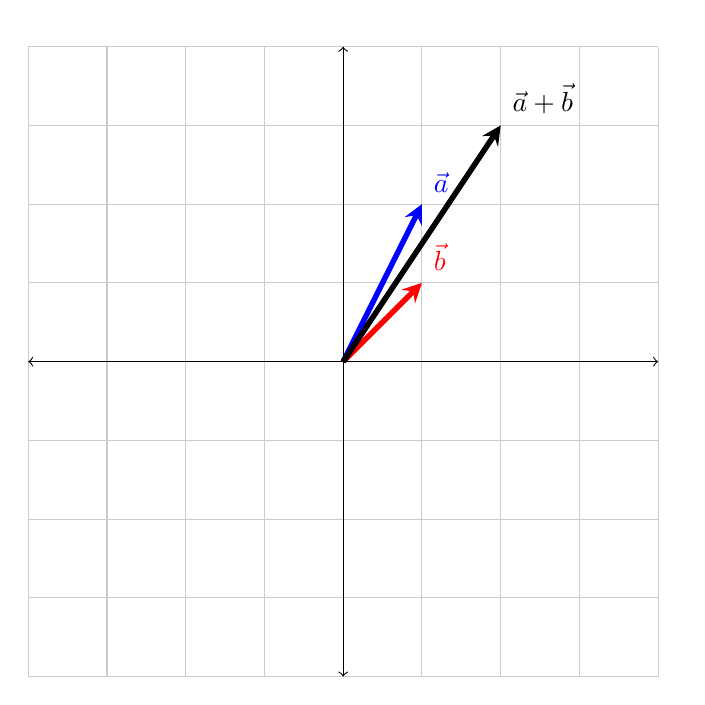
\begin{tikzpicture}
    \draw[thin, gray!40] (-4,-4) grid (4,4);
    \draw[line width=2pt, blue, -stealth] (0,0) -- (1,2) node[anchor=south west]{\(\vec{a}\)};
    \draw[line width=2pt, red, -stealth] (0,0) -- (1,1) node[anchor=south west]{\(\vec{b}\)};
    \draw[line width=2pt, black, -stealth] (0,0) -- (2,3) node[anchor= south west]{\(\vec{a} + \vec{b}\)};
    \draw[<->] (-4,0) -- (4,0) node[right]{\(\ihat\)};
    \draw[<->] (0,-4) -- (0,4) node[above]{\(\jhat\)};
  \end{tikzpicture}
  \caption{Illustration of vector addition.}
  \label{vecadd}
\end{figure}



Let us analyze \Cref{vecadd}. Firstly, notice that \(\vec{a}=1 \ihat + 2 \jhat\) and \(\vec{b}=1 \ihat + 1 \jhat\). Thus, \(\vec{a}+\vec{b}=2 \ihat + 3 \jhat\), exactly like in our figure. One way to understand this is to "attach" the vector \(\vec{a}\)'s tail to \(\vec{b}\)'s head.
\begin{marginfigure}
  \centering
  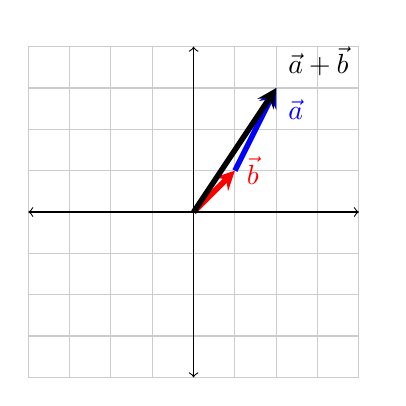
\begin{tikzpicture}[scale=0.525]
    \draw[thin, gray!40] (-4,-4) grid (4,4);
    \draw[line width=2pt, blue, -stealth] (1,1) -- (2,3) node[anchor=north west]{\(\vec{a}\)};
    \draw[line width=2pt, red, -stealth] (0,0) -- (1,1) node[anchor=west]{\(\vec{b}\)};
    \draw[line width=2pt, black, -stealth] (0,0) -- (2,3) node[anchor= south west]{\(\vec{a} + \vec{b}\)};
    \draw[<->] (-4,0) -- (4,0) node[right]{\(\ihat\)};
    \draw[<->] (0,-4) -- (0,4) node[above]{\(\jhat\)};
  \end{tikzpicture}
  \caption{Illustration of vector "head to tail" addition.}
  \label{vecaddattach}
\end{marginfigure}
You may have seen this in your physics class before. Similarly, the subtraction of vectors \(\vec{x}=
\begin{bsmallmatrix}
  a \\
  b
\end{bsmallmatrix}
\) and \(\vec{y}=
  \begin{bsmallmatrix}
    c \\
    d
  \end{bsmallmatrix}
\) is \(\vec{x}-\vec{y}=
\begin{bsmallmatrix}
  a - c \\
  b - d
\end{bsmallmatrix}
\). Of course, we can use the same "head to tail" model to explain vector subtraction. Subtracting \(\vec{y}\) from \(\vec{x}\) is simply finding the vector whose tail is on the head of \(\vec{y}\) and whose head is on the head of \(\vec{x}\).
